\documentclass{article}
\usepackage[utf8]{inputenc}
\usepackage{listings}
\usepackage{color}
\usepackage{tikz}
\usetikzlibrary{shapes}

\definecolor{dkgreen}{rgb}{0,0.6,0}
\definecolor{gray}{rgb}{0.5,0.5,0.5}
\definecolor{mauve}{rgb}{0.58,0,0.82}

\lstset{frame=tb,
  language=C,
  aboveskip=3mm,
  belowskip=3mm,
  showstringspaces=false,
  columns=flexible,
  basicstyle={\small\ttfamily},
  numbers=none,
  numberstyle=\tiny\color{gray},
  keywordstyle=\color{blue},
  commentstyle=\color{dkgreen},
  stringstyle=\color{mauve},
  breaklines=true,
  breakatwhitespace=true,
  tabsize=3
}

\begin{document}

\title{Relat\'orio Fase II}
\author{Andr\'e Camargo Perello - 9912403\\Lucas Henrique Bahr Yau - 9763832\\Rud\'a Lima da Floresta - 9912410}
\date{}

\maketitle
\newpage
\begin{itemize}
    \item \textbf{Introdu\c c\~ao} \\
    Nesta fase do projeto devemos, utilizando o c\'odigo que interpreta c'odigo de cada rob\^o fornecido pelo usu\'ario, inserir novos comandos e criar estruturas para que a base do jogo esteja formada. Dentre elas est\~ao os tipos de \textbf{terreno}, o \textbf{Grid Hexagonal}, uma matriz onde o jogo se passar\'a, \textbf{chamadas de sistema}, onde o rob\^o pede ao sistema para realizar uma a\c c\~ao, \textbf{cria\c c\~ao e destrui\c c\~ao de ex\'ercitos} de rob\^os e um atualizador do jogo, ou \textbf{game loop}.
    
    \item \textbf{Arena} \\
    A Arena \'e onde o jogo ocorre. Sua implementa\c \~ao envolve uma \textit{struct} que cont\'em o Grid Hexagonal, representando o tabuleiro, um vetor que armazena os ex\'ercitos assim como dois inteiros, um representando a \'ultima posi\c c\~ao livre do vetor de ex\'ercitos e outro representando o tempo decorrido de jogo.
    \begin{lstlisting}
        // Arena
        typedef struct {
          Grid grid;
          int rows;
          int cols;
          int tempo;
          Maquina* exercitos[MAXMEM];
          int firstFree;
        } Arena;

    \end{lstlisting}
    \item \textbf{C\'elula} \\
    Uma C\'elula \'e uma struct da forma:
    \begin{lstlisting}
        // Celula
        typedef struct {
          Terreno t;
          Base b;
          Cristais c;
          Ocupacao o;
        } Celula;
    
    \end{lstlisting}
    Com esses dados, listamos o que cada c\'elula do Grid necessita para que o jogo funcione bem. Assim como \'e dedut\'ivel, o \textit{Terreno t} indica que tipo de terreno a c\'elula possui. A \textit{Base b} determina se a c\'elula configura uma base e se \'e amiga ou inimiga. \textit{Cristais c} \'e um inteiro que possui o n\'umero de cristais contidos na c\'elula. Por \'ultimo, a \textit{Ocupa\c \~ao o} diz se a c\'elula est\'a ocupada e se quem a ocupa \'e amigo ou inimigo.
    
    \item \textbf{Grid Hexagonal} \\
    O Grid Hexagonal \'e apenas uma matriz de c\'elulas onde o jogo ser\'a realizado. Ele est\'a definido da forma:
    \begin{lstlisting}
        typedef struct Celula** Grid;
    
    \end{lstlisting}
    Ele \'e inicializado da forma:
    \begin{lstlisting}
    arena->grid = malloc(nrows * sizeof(Grid *));
	for(int i = 0; i < nrows; i++) {
	    arena->grid[i] = malloc(ncolumns * sizeof(Grid));
	\end{lstlisting}
	
	Al\'em disso inicializamos o tipo do terreno e a quantidade de cristais aleatortiamente para toda c\'elula do grid. Por simplicidade, as bases de cada time começam nos cantos superior esquerdo e inferior direito, sendo os \'unicos lugares onde h\'a ocupa\c c\~ao.\\
	Optamos por utilizar o grid como na imagem abaixo:\\
	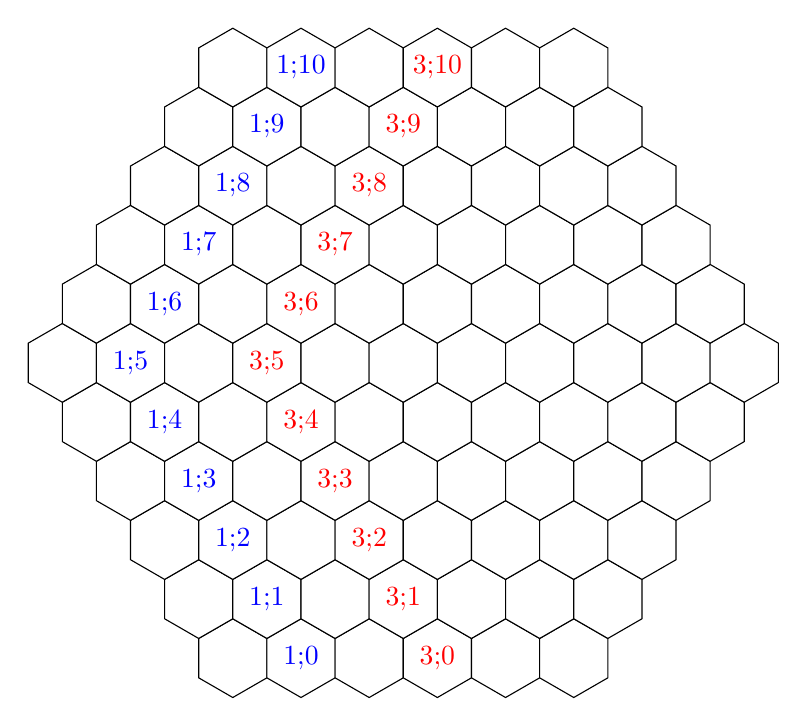
\begin{tikzpicture} [hexa/.style= {shape=regular polygon,regular polygon sides=6,minimum size=1cm, draw,inner sep=0,anchor=south,fill=white,rotate=30}]
    \foreach \j in {0,...,5}{%
        \pgfmathsetmacro\end{5+\j} 
        \foreach \i in {0,...,\end}{%
            \node[hexa] (h\i;\j) at ({(\i-\j/2)*sin(60)},{\j*0.75}) {};}  }      
    \foreach \j in {0,...,4}{%
        \pgfmathsetmacro\end{9-\j} 
        \foreach \i in {0,...,\end}{%
            \pgfmathtruncatemacro\k{\j+6}  
            \node[hexa] (h\i;\k) at ({(\i+\j/2-2)*sin(60)},{4.5+\j*0.75}) {};}  } 

  \foreach \k in {0,...,10}  {\node [circle,red,minimum size=1cm] at (h3;\k) {3;\k};} 
   \foreach \k in {0,...,10}  {\node [circle,blue,minimum size=1cm] at (h1;\k) {1;\k};}   
\end{tikzpicture}

    Isso facilitou a implementa\c cao de movimentos e o acesso \`as celulas vizinhas.
    \item \textbf{Game Loop} \\
    Esta \'e fun\c \~ao respons\'avel pela atualiza\c c\~ao do jogo do tempo $t$ para o tempo $t+1$:
    \begin{lstlisting}
    void atualiza(Arena *arena, int ciclos);
    
    \end{lstlisting}
    Nada mais que um \textit{loop} que percorre o vetor de rob\^os da Arena e executa as instru\c c\~oes fornecidas ao rob\^o um n\'umero \textit{ciclos} de vezes, aumentando o tempo de jogo em 1 a cada atualiza\c c\~ao.\\
    Dessa forma, o \textit{game loop} \'e formado por uma s\'erie de chamadas desta fun\c c\~ao, utilizadas at\'e que um dos times saia vencedor.
    
    \item \textbf{O tipo OPERANDO} \\
    Antes de falarmos sobre as chamadas de sistema e o m\'etodo ATR, pe\c cas vitais para o funcionamento do programa nesta fase, devemos nos ater \`as escolhas que foram feitas para a implementa\c c\~ao do tipo \textbf{OPERANDO}. \\
    A \textbf{struct OPERANDO} \'e da forma: 
    \begin{lstlisting}
    typedef struct {
        int n;
        Direction d;
    } OPERANDO;
    \end{lstlisting}
    Esta escolha de implementa\c c\~ao se baseou nos variados tipos de programas que um rob\^o pode ter. Sejam calcular fatoriais, obter informa\c c\~oes sobre uma c\'elula do grid ou mover-se e atacar, as instru\c c\~oes precisam apenas de dois tipos de informa\c c\~ao, um inteiro ou uma dire\c c\~ao. Para ilustrar isso, considere o seguinte programa:
    \begin{lstlisting}
        ACAO  MOVE WEST
        ACAO  ATTK SWEST
        INTER PUSH NEAST
        NUM   ATR  0
    \end{lstlisting}
    Embora estes comandos n\~ao tenham sido explicados at\'e o momento, \'e facil ver que ele consiste em:
    \begin{itemize}
        \item Mover-se na dire\c c\~ao oeste
        \item Atacar na dire\c c\~ao sudeste
        \item Inserir na pilha a c\'elula na dire\c c\~ao nordeste
        \item Empilhar o primeiro atributo da c\'elula inserida na pilha
    \end{itemize}
    Como a pilha que executa o rob\^o consiste em uma pilha de tipo OPERANDO, essa implementa\c \~ao facilitou uma s\'erie de problemas que encontramos, e poder\'iamos encontrar, devido a outras implementa\c c\~oes que se baseavam em tornar o OPERANDO um tipo de c\'elula do grid. Deste modo, lidamos apenas com inteiros e uma enumera\c c\~ao das dire\c c\~oes poss\'iveis do grid hexagonal.
    
    \item \textbf{System Calls} \\
    As chamadas de sistema s\~ao um conjunto de fun\c c\~oes que, dados \textit{a\c c\~ao} e \textit{dire\c c\~ao}, verifica se \'e uma a\c c\~ao v\'alida e executa no rob\^o que a pediu Elas retornam um OPERANDO que possui na sua parcela inteira um indicativo do sucesso ou fracasso da chamada. Este OPERANDO \'e empilhado para que o rob\^o possa fazer verifica\c c\~oes e estruturas mais complexas de decis\~ao. Dentre as a\c c\~oes poss\'iveis est\~ao: \textit{mover, pegar, atacar, depositar}. Logo, o usu\'ario faz uma chamada da forma:
    \begin{lstlisting}
        ACAO <ACTION> <DIRECTION>
    \end{lstlisting}
    Temos as a\c c\~oes:
    \begin{enumerate}
        \item MOVE
        \begin{lstlisting}
        OPERANDO moveMachine(Arena *A, Maquina *m, Direction d);
        \end{lstlisting}
        Esta fun\c c\~ao apenas "olha" se a posi\c c\~ao correspondente a dire\c c\~ao \textit{d} est\'a ocupada e atualiza a posi\c c\~ao atual do rob\^o caso contr\'ario.
        
        \item GRAB
        \begin{lstlisting}
        OPERANDO grabCrystal(Arena *A, Maquina *m, Direction d);
        \end{lstlisting}
        Esta fun\c c\~ao apenas verifica se a posi\c c\~ao correspondente a dire\c c\~ao \textit{d} possui cristais e diminui a quantidade de cristais da c\'elula em uma unidade, aumentando a do rob\^o na mesma propor\c c\~ao.
        
        \item DEPO
        \begin{lstlisting}
        OPERANDO depositCrystal(Arena *A, Maquina *m, Direction d);
        \end{lstlisting}
        Esta fun\c c\~ao retira cristal do rob\^o e aumenta a da c\'elula, amos em uma unidade.
        \item ATTK
        \begin{lstlisting}
        OPERANDO attackMachine(Arena *A, Maquina *m, Direction d);
        \end{lstlisting}
        Esta fun\c c\~ao apenas verifica se h\'a um rob\^o do time inimigo na posi\c c\~ao correspondente e, por enquanto, se houver, imprime uma mensagem na sa\'ida padr\~ao. Futuramente pretendemos implementar um sistema de pontos de vida nos rob\^os, al\'em de pontos de ataque e defesa para que esta fun\c c\~ao se mostre \'util.
    \end{enumerate}
    
    \item \textbf{O m\'etodo ATR} \\
    Antes de chegarmos ao m\'etodo ATR, vale a pena explicar como funciona para o usu\'ario empilhar uma c\'elula para que ele possa acessar um de seus atributos. \\
    Criamos um tipo novo de instru\c c\~ao que possui aepenas uma chamada espec\'ifica:
    \begin{lstlisting}
        INTER PUSH <DIRECTION>
    \end{lstlisting}
    De nome \textbf{intera\c c\~ao}, esta instru\c c\~ao empilha um OPERANDO com a dire\c c\~ao especificada para que esta dire\c c\~ao possa ser utilizada pelo m\'etodo ATR atrav\'es da fun\c c\~ao:
    \begin{lstlisting}
        getPosition(Maquina *m, Direction d, int *i, int *j, int rows, int cols);
    \end{lstlisting}
    Esta fun\c c\~ao rececbe a dire\c c\~ao especificada e coloca nos ponteiros i e j a posi\c c\~ao correspondente no grid.
    Assim como especificado, quando o usu\'ario chama ATR, a seguinte parcela de c\'odigo \'e executada:
    \begin{lstlisting}
        case ATR:
			tmp = desempilha(pil);
			int i = -1, j = -1;
			getPosition(m, tmp.d, &i, &j, arena->rows, arena->cols);
			if(i != -1){
				switch(arg.n){
				    case 0:
						tmp.n = (int)(arena->grid[i][j].t);
						empilha(pil, tmp);
						break;
					case 1:
						tmp.n = (int)(arena->grid[i][j].b.isBase);
						empilha(pil, tmp);
						break;
					case 2:
				    	tmp.n = (int)(arena->grid[i][j].c);
						empilha(pil, tmp);
						break;
					case 3:
						tmp.n = (int)(arena->grid[i][j].o.ocupado);
						empilha(pil, tmp);
						break;
				}
			}
			else
				printf("Celula invalida.\n");
    \end{lstlisting}
    Ou seja, pegamos o atributo de n\'umero arg.n, especificado pelo usu\'ario, e empilhamos. Um detalhe vital para a simplifica\c c\~ao da implementa\c c\~ao consiste nos atributos \textit{Base} e \textit{Ocupacao}. Ambas as structs possuem duas informa\c c\~oes, por\'em optamos por indicar ao usu\'ario apenas se a c\'elula correspondente \'e base ou se est\'a ocupada.\\
    
    \item \textbf{Cria\c c\~ao e destrui\c \~ao de ex\'ercitos} \\
    Essas fun\c c\~oes s\~ao simples varreduras pelo vetor de rob\^os da arena. Para fins de simplifica\c c\~ao, limitamos a quantidade de rob\^os da arena em 100, o que explica as constantes nas fun\c c\~oes. No momento inserimos uma quantidade size de rob\^os de um determinado time e colocamos sua posi\c c\~ao inicial na primeira posi\c c\~ao v\'alida do grid. Isto mudar\'a nas fases futuras, pois estamos colocando todos os rob\^os, de times diferentes, na mesma localiza\c c\~ao.
    \begin{lstlisting}
        void InsereExercito(Arena *arena, int size, INSTR *p, Time team) {

          	if(size > 100-arena->firstFree) {
          		printf("The Arena is full.\n");
          		return;
          	}
          	
        	for(int i = arena->firstFree; i < size + arena->firstFree; i++){
        		Maquina *robo;
        		robo = cria_maquina(p);
        		
        		robo->t = team;
        		arena->exercitos[i] = robo;
        		robo->crystals = 0;
        		robo->alive = True;
        		robo->x = 1;
        		robo->y = 0;
        		
        	}
        	arena->firstFree += size;
        	
        }
    \end{lstlisting}
    
    Decidimos por destruir um grupo de rob\^os utilizando o time que ele pertence.
    \begin{lstlisting}
    void removeExercito(Arena *arena, Time t) {
    
    	for(int i = 0; i < arena->firstFree; i++) {
    		if(arena->exercitos[i] != NULL && arena->exercitos[i]->t == t) {
    			arena->exercitos[i] = NULL;
    		}
    	}
    
    
    	arena->firstFree = tapaBuraco(arena->exercitos, arena->firstFree);
    }	
    \end{lstlisting}
    A fun\c c\~ao \textit{tapaBuraco} foi essencial para a solu\c c\~ao de bugs e para a atualiza\c c\~ao da primeia posi\c c\~ao livre do vetor de m\'aquinas. Ela funciona similarmente \`a fun\c c\~ao \textit{partition} do \textit{quicksort} que, dado um piv\^o, separa todos os elementos do vetor em maiores que o piv\^o e menores que ele. Neste caso, separamos todos os ponteiros \textbf{NULL} pra m\'aquina daqueles que n\~ao o s\~ao
    
    \item \textbf{O montador} \\
    O programa em python do montador simplesmente gera um arquivo em C a partir de um programa feito para um rob\^o como no exemplo:
    \begin{lstlisting}
    recursiveFactorial:
    
      NUM PUSH 9 
      NUM CALL 4
      NUM PRN 0
      NUM END 0
      NUM ALC 1
      NUM DUP 0
      NUM STL 0
      NUM PUSH 1
      NUM EQ 0
      NUM JIF 13
      NUM PUSH 1
      NUM FRE 1
      NUM RET 0
      NUM RCE 0
      NUM PUSH 1
      NUM SUB 0
      NUM CALL 4
      NUM RCE 0
      NUM MUL 0
      NUM FRE 1
      NUM RET 0
    \end{lstlisting}
    
    A diferen\c ca principal do c\'odigo da fase anterior est\'a no vetor de instru\c c\~oes prog gerado pelo montador. Como adaptamos o tipo operando, o montador agora verifica de que tipo \'e o comando da linha especificada e acrescenta uma dire\c c\~ao \textit{default} ou um inteiro \textit{default}:
    
    \begin{lstlisting}
    INSTR prog[] = {
    
    
      {NUM, PUSH, { 9, WEST }},
      {NUM, CALL, { 4, WEST }},
      {NUM, PRN, { 0, WEST }},
      {NUM, END, { 0, WEST }},
      {NUM, ALC, { 1, WEST }},
      {NUM, DUP, { 0, WEST }},
      {NUM, STL, { 0, WEST }},
      {NUM, PUSH, { 1, WEST }},
      {NUM, EQ, { 0, WEST }},
      {NUM, JIF, { 13, WEST }},
      {NUM, PUSH, { 1, WEST }},
      {NUM, FRE, { 1, WEST }},
      {NUM, RET, { 0, WEST }},
      {NUM, RCE, { 0, WEST }},
      {NUM, PUSH, { 1, WEST }},
      {NUM, SUB, { 0, WEST }},
      {NUM, CALL, { 4, WEST }},
      {NUM, RCE, { 0, WEST }},
      {NUM, MUL, { 0, WEST }},
      {NUM, FRE, { 1, WEST }},
      {NUM, RET, { 0, WEST }},
    
    };
    
    \end{lstlisting}
    
    \item \textbf{Dificuldades} \\
    A maior dificuldade nesta fase foi com o tratamento de vari\'aveis de diferentes tipos. Como a especifica\c c\~ao n\~ao era muito clara, focamos em entregar um produto que possui as funcionalidades pedidas. Em especial, lidar com a struct OPERANDO foi um jogo de acertos e erros at\'e encontrar a implementa\c c\~ao que mais fizesse sentido e que gerasse o menor n\'umero de bugs. 
    
    \item \textbf{Makefile e Testes} \\
    Este \'e o c\'odigo do nosso \textbf{Makefile}:
    \begin{lstlisting}
            # Variáveis #################################################
        CC = gcc
        CFLAGS = -std=c99
        EXECS = testAttackMachine testAtualiza testDepositCrystal testGetPosition testGrabCrystal testHasCrystal testInicializaGrid testInsereExercito testRemoveExercito testRemoveMortos testSysCall testTapaBuraco testMove
        OBJ = testAttackMachine.o testAtualiza.o testDepositCrystal.o testGetPosition.o testGrabCrystal.o testHasCrystal.o testInicializaGrid.o testInsereExercito.o testRemoveExercito.o testRemoveMortos.o testSysCall.o testTapaBuraco.o testMove.o
        HEADERS = maq.h arena.h structures.h instr.h pilha.h
        DEPENDS = maq.c arena.c pilha.c
        
        
        
        # Cria os arquivos-objeto de todos os testes ################
        %.o: %.c $(CFLAGS) $(HEADERS)
        	$(CC) -c $(CFLAGS) -o $@ $<
        
        
        
        # Compila todos os arquivos-objetos #########################
        all: $(OBJ)
        	gcc $(CFLAGS) -o testAttackMachine testAttackMachine.o $(DEPENDS)
        	gcc $(CFLAGS) -o testAtualiza testAtualiza.o $(DEPENDS)
        	gcc $(CFLAGS) -o testDepositCrystal testDepositCrystal.o $(DEPENDS)
        	gcc $(CFLAGS) -o testGetPosition testGetPosition.o $(DEPENDS)
        	gcc $(CFLAGS) -o testGrabCrystal testGrabCrystal.o $(DEPENDS)
        	gcc $(CFLAGS) -o testHasCrystal testHasCrystal.o $(DEPENDS)
        	gcc $(CFLAGS) -o testInicializaGrid testInicializaGrid.o $(DEPENDS)
        	gcc $(CFLAGS) -o testInsereExercito testInsereExercito.o $(DEPENDS)
        	gcc $(CFLAGS) -o testMove testMove.o $(DEPENDS)
        	gcc $(CFLAGS) -o testRemoveExercito testRemoveExercito.o $(DEPENDS)
        	gcc $(CFLAGS) -o testRemoveMortos testRemoveMortos.o $(DEPENDS)
        	gcc $(CFLAGS) -o testSysCall testSysCall.o $(DEPENDS)
        	gcc $(CFLAGS) -o testTapaBuraco testTapaBuraco.o $(DEPENDS)
        
        
        
        # CLEAN #####################################################
        clean:
        	rm -f $(EXECS) *.o
    \end{lstlisting}
    
    Este file ajuda o monitor a compilar todos os testes com apenas um comando. Dessa forma, pode apenas testar cada um deles. Cada teste possui um modo de testar suas sa\'idas que, em sua maioria, est\~ao especificadas no file de teste. 
    Caso o monitor queira gerar um programa para testar nosso c\'odigo, basta gerar o c\'odigo com o aux\'ilio do programa \textit{montador.py} que gera o c\'odigo em C a ser executado.
    
    \item \textbf{Conclus\~oes} \\
    Embora hajam funcionalidades que poderiam ser melhor lapidadas, como a introdu\c c\~ao de um ex\'ercito de um determinado time na arena, optamos por simplificar a implementa\c c\~ao para poder lidar melhor com detalhes nas fases seguintes. Assim, todas as funcionalidades pedidas operam de acordo e podem ser reutilizadas e ampliadas a medida que o projeto se desenvolve. \\
    Em suma, temos um esqueleto bem estruturado, por\'em feito de ossos, n\~ao de diamantes.

\end{itemize}
\end{document}
